\chapter{Modulateur sigma-delta}
Le modulateur sigma-delta se trouve à la suite du filtre et avant l'amplifacteur de classe D. Ce bloc a pour but de moduler le signal d'entrée (un pseudo sinus) par largeur d'impulsion, c'est-à-dire en signal carré de valeurs seuils constantes mais de fréquence variable dont la valeur moyenne est égale à la valeur absolue du signal initial. L'obtention d'un signal composé de deux états est nécessaire pour une utilisation optimale en terme de puissance de l'amplificateur de classe D. (........)

%\begin{figure}[ht]
%	\centering
%	\includegraphics[scale=0.7]{....}
%	\caption{Entré et sortie du sigma-delta}
%	\label{fig:entrée-sortie-sigma-delta}
%\end{figure}

\section{Fonctionnement du système}

La fréquence de commutation (....) du sigma-delta est supposée très élevée par rapport au signal d'entrée. Ceci permet de considérer le signal d'entrée continu de façon locale.


Voici ci-dessous le schéma bloc du sigma-delta.

\begin{figure}[ht]
	\centering
	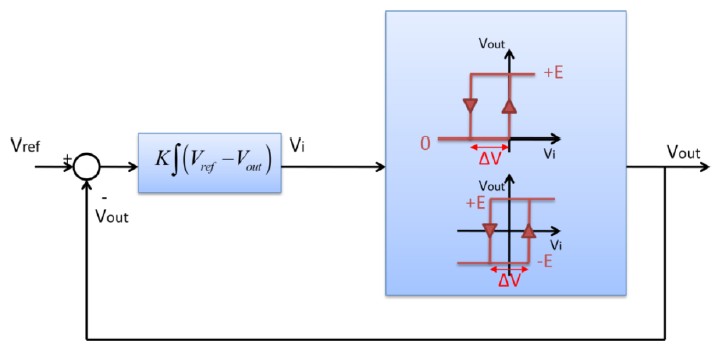
\includegraphics[scale=0.7]{img-sigma-delta/schema-blocs.png}
	\caption{Schéma bloc du modulateur sigma-delta.}
	\label{fig:sigma-delta-schema-blocs}
\end{figure}

Ce bloc est constitué de deux parties distinctes : un intégrateur et une bascule asymétrique.
L'intégrateur est caractérisé par un coefficient d'intégration K. La bascule est elle caractérisée par deux tensions de basculement : $V_H$, la tension de basculement haute  fixée arbitrairement à 0 et $V_L$, la tension de basculement basse avec $\Delta V = V_H - V_L$, ainsi que des valeurs seuils de sortie : $V_{\text{outH}} = E$, la tension de sortie haute, et la tension $V_{\text{outL}} = 0$. $V_{\text{outL}}$ est fixée à 0 car l'amplificateur de classe D nécessite en entré une tension positive ($E$), ou 0.

La période d'oscillation du signal de sortie (qui est 
identique à la période d'oscillation du signal intermédiaire
$V_I$ sur la figure \ref{fig:sigma-delta-schema-blocs})
se calcule en effectuant le raisonnement suivant.
Initialement, soit $V_{\text{ref}}$ positif et
$V_{\text{out}} = 0$. $V_I$ est alors immédiatement positif
et $V_{\text{out}}$ sature directement à $E$. Comme $V_{\text{ref}}$
est $\leq E$, $V_I$ va maintenant décroître jusqu'à atteindre
$\Delta V$. A ce moment précis, $V_{\text{out}} = 0$
et donc $V_I$ va croître jusqu'à atteindre 0, et ainsi de suite.

De là s'obtiennent le temps de descente $t_f$ et le temps de montée $t_r$
du signal $V_I$\footnote{Ce signal sera soit un signal triangulaire,
soit un signal en dents de scie, selon la valeur de $V_{\text{ref}}$.}
\[ t_f = -\frac{\Delta V}{(V_{\text{ref}} - E)K},\]
\[ t_r = \frac{\Delta V}{KV_{\text{ref}}}.\]
La période $T$ étant la somme du temps de descente et du temps
de montée, elle est donnée par
\[ T = \frac{\Delta V}{K}\left(\frac{1}{V_{\text{ref}}} - \frac{1}{V_{\text{ref}} - E}\right) \]
et donc finalement
\begin{equation} 
	f = -\frac{K}{\Delta V} \frac{V_{\text{ref}}(V_{\text{ref}}-E)}{E}.
	\label{eq:sigma-delta-frequency}
\end{equation}

\paragraph{Remarque}
A partir du temps de descente et du temps de montée, nous
pouvons prouver que la moyenne du signal carré $V_{\text{out}}$
vaut bien $V_{\text{ref}}$. Il suffit de démontrer l'égalité
suivante
\[ \frac{E \cdot t_f + 0 \cdot t_r}{T} = V_{\text{ref}}.\]

La fréquence en fonction de $V_{\text{ref}}$ est donc
une parabole avec une racine en \unit{0}{\volt} et une
racine en \unit{E}{\volt}.

La fréquence de sortie maximale est atteinte pour 
$V_{\text{ref}} = \frac{E}{2}$ et vaut
\[ f_{\text{max}} = \frac{K}{\Delta V}\frac{E}{4}. \]
Le sigma-delta doit remplir certaines spécifications afin de remplir son rôle au sein du système global : \begin{enumerate}
\item Le signal de sortie ne peut pas atteindre de fréquence nulle pour la gamme d'amplitude du signal d'entrée car la valeur moyenne du signal de sortie ne correspondrait pas au signal d'entrée pour ces deux racines.
\item La fréquence de sortie du sigma-delta doit respecter le théorème d'échantillonage de Shannon, c'est-à-dire que la fréquence de sortie doit être au minimum deux fois supérieure à la fréquence maximale du signal d'entrée afin de permettre la reconstitution du signal d'entrée.
\item La fréquence maximale d'entrée de l'amplificateur de classe D est de 100kHz.
\item La bascule ne doit pas être sensible au bruit, $V_{\text{ref}}$ ne doit donc pas être trop faible.
\end{enumerate}

Afin de répondre à ces conditions, la fréquence maximale de sortie est fixée à 80kHz. La parabole (fréquence de sortie/amplitude d'entrée) est centrée autour de l'origine car le signal d'entrée est centrée en 0 et les racines de celles-ci se situent en +15V et -15V. Ainsi, la gamme d'amplitude de tension d'entrée étant de -3V à 3V la fréquence de sortie n'est jamais nulle. De plus, la fréquence maximale du signal d'entrée étant de 8kHz, la fréquence du signal de sortie est bien supérieure au double de cette fréquence pour l'ensemble de la gamme d'amplitude. $V_{\text{ref}}$ est fixé arbitrairement à $1V$.

La figure ci-dessous illustre la réponse en fréquence établie et met en évidence la limite induit par le théorème de Shannon ainsi que la gamme utiliser par notre système.
\begin{figure}[ht]
	\centering
	%\includegraphics[scale=0.6]{GRAPHE1MATLAB.png}
	\caption{Fréquence de sortie en fonction de la tension d'entrée et contraintes}
	\label{fig:de}
\end{figure}
Il est possible de constater que la zone utilisée est nettement inférieure à la zone exploitable. Cela sera mis plus en avant dans la section %(\f !!!!!!!!).

\section{Dimensionnement et circuit réel}
Le circuit du modulateur sigma-delta est représenté
à la figure \ref{fig:sigma-delta-circuit}.

\begin{figure}[ht]
	\centering
	%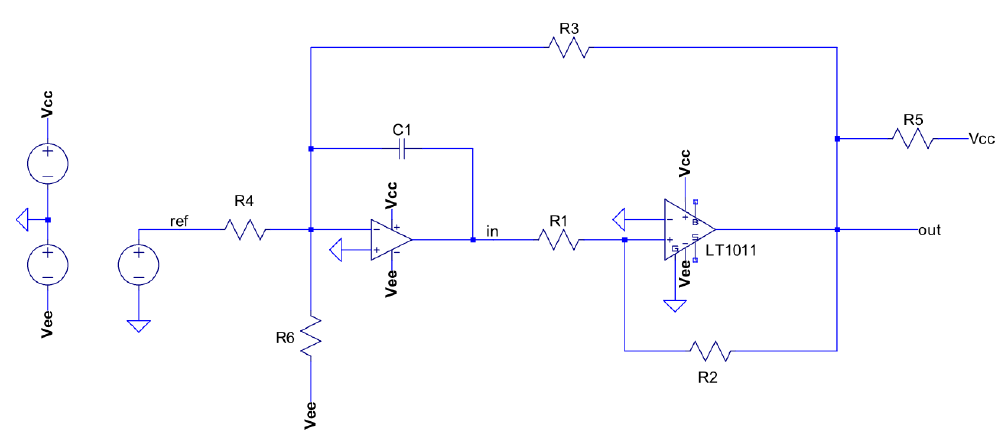
\includegraphics[scale=0.6]{img-sigma-delta/sigma-delta-circuit.png}
	\caption{Circuit du modulateur.}
	\label{fig:sigma-delta-circuit}
\end{figure}

La résolution de ce circuit permet d'obtenir des équations
de la même forme que celles de la figure
\ref{fig:sigma-delta-schema-blocs}.
L'amplificateur opérationnel étant connecté en contre-réaction,
sa bornée d'entrée est virtuellement à la masse : $v_- = v_+ = 0$.
Les différents courants dans le circuit sont alors donnés par
\[ i_{R_4} = \frac{V_{\text{ref}}}{R_4},\]
\[ i_{R_6} = \frac{V_{\text{ee}}}{R_6},\]
\[ i_{R_3} = \frac{V_{\text{out}}}{R_3},\]
\[ i_{C_1} = -C_1\fdif{v_{\text{in}}}{t}.\]
KCL permet ensuite d'écrire l'équation suivante
\[ i_{C_1} = i_{R_4} + i_{R_6} + i_{R_3}\]
et donc d'obtenir
\[ v_{\text{in}} = -\frac{1}{C_1}\int \frac{V_{\text{ref}}}{R_4}
+ \frac{V_{\text{ee}}}{R_6} + \frac{V_{\text{out}}}{R_3}.\]
Pour se ramener à l'équation de la figure
\ref{fig:sigma-delta-schema-blocs}, on
$V'_{\text{ref}} = -R_3(\frac{V_{\text{ref}}}{R_4}+\frac{V_{\text{ee}}}{R_6})$
pour enfin obtenir
\[ v_{\text{in}} = \frac{1}{C_1R_3} \int V'_{\text{ref}} - V_{\text{out}}\]
où $V'_{\text{ref}}$ correspond au $V_{\text{ref}}$
de la figure \ref{fig:sigma-delta-schema-blocs}.

Pour dimensionner le modulateur, plusieurs contraintes doivent
être respectées. Premièrement la fréquence maximale doit être
de \unit{80}{\kilo\hertz}. Et deuxièment, la parabole doit s'étendre
de manière à ce que ces racines soient \unit{-15}{\volt} et
\unit{+15}{\volt}. Enfin, $\Delta V$ doit être choisit de manière
à ce que la bascule ne soit pas sensible au bruit.

Nous allons directement anticiper une non-idéalité de la bascule,
la valeur de saturation $E$ n'est pas égale à la tension
d'alimention. Nous avons plutôt $E \approx$ \unit{13.5}{\volt}.

Pour centrer la parabole, il faut que $\frac{R_3}{R_6}V_{\text{ee}}$
soit égale à \unit{6.75}{\volt}. Il faut ensuite étirer la
parabole de manière à ce que ses racines soient $\pm$\unit{15}{\volt}.
Il faut donc $\frac{R_3}{R_4} = 0.45$. 

En utilisant des valeurs de composants standards (série de Renard E12), 
nous pouvons choisir, $R_3 =$ \unit{22}{\kilo\ohm} et $R_4 = R_6 =
$ \unit{48.5}{\kilo\ohm}.

Passons ensuite à la contrainte sur la fréquence. Nous avons la 
relation suivante:
\[ \frac{K}{\Delta V}\frac{E}{4} = 80000.\]
Nous pouvons fixer arbitrairemet $\Delta V$ à \unit{1}{\volt}. Nous avons alors
$K = \frac{1}{C_1R_3} = 23703.7037$ et donc $C1 =$ \unit{1.9}{\nano\farad}.
Enfin, comme $\Delta V = \frac{R_1}{R_2}E$, nous pouvons par exemple
choisir $R_1 =$ \unit{10}{\kilo\ohm} et $R_2 =$ \unit{134.6}{\kilo\ohm}.

% TODO : on peut sans doute réaliser encore un meilleur
% dimensionnement en considérant dans les calculs les valeurs
% exactes (je veux dire par là les valeurs mesurées sur circuit,
% pas les valeurs théoriques) OU utiliser un système de calibrage

Pour appliquer la signal de sortie du modulateur
à l'étage suivant du circuit, il faudra utiliser un diviseur
résistif car l'étage suivant ne supporte pas des entrées supérieures
à \unit{5}{\volt}.

\section{Confrontation des mesures et de la théorie}
En superposant le graphe théorique que nous pouvons obtenir avec les valeurs
obtenues dans la section précédente
et des mesures effectuées sur une implémentation en circuit
du modulateur, nous obtenons la figure \ref{fig:sigma-delta-f-vs-vref-dim-vs-real}.

\begin{figure}[ht]
	\centering
	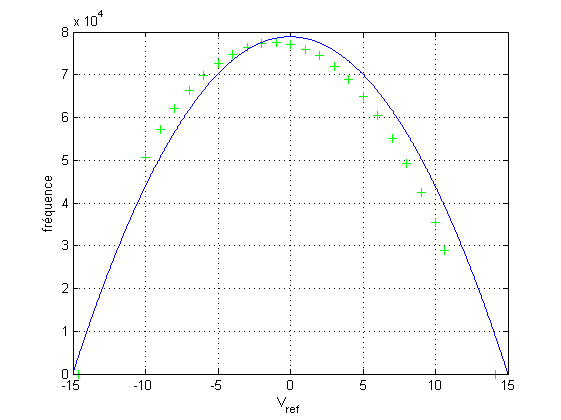
\includegraphics[scale=0.6]{img-sigma-delta/sigma-delta-f-vs-vref-dim-vs-real.png}
	\caption{En bleu, les prévisions théoriques et en vert les mesures.}
	\label{fig:sigma-delta-f-vs-vref-dim-vs-real}
\end{figure}

Nous constatons que la théorie colle assez bien à la réalité. Le
faible décalage dépend sans doute des tolérances des résistances,
des variations dans les alimentations (le MyDAQ sort, dans ce cas, du
\unit{+14.10}{\volt} et du \unit{-14.62}{\volt} plutôt que du
$\pm$\unit{15}{\volt}), des variations dans la valeur de saturation
$E$ ($\approx$ \unit{13.62}{\volt}). Nous pourrions effectuer un
dimensionnement plus précis à partir de ces valeurs réelles afin
d'obtenir une prévision théorique encore plus proche de la réalité.
% FIXME (à confirmer)
Le problème, c'est que les valeurs des tensions
d'alimentation (par exemple) dépendent justement de la charge 
connectée, et donc du choix des résistances effectuées lors du dimensionnement.